\chapter{Python GUI Using qudi}

\section{Objective}

The objective of the second phase of the internship was to develop an embedded system interface enabling users to control the \acs{quEDU} system according to their specific requirements. This involved the creation of a Python API using the clientLib, which provides a range of control functions for device management. Furthermore, the project was extended by developing a Python-based graphical user interface (GUI) to offer a more intuitive and user-friendly experience. The integration and functionality of both the API and \acs{GUI} were tested using custom examples to ensure seamless operation and user satisfaction.

\section{\acs{quEDU} - The Science Kit for Quantum Education}

The \acs{quEDU} serves as a comprehensive platform for conducting a wide range of quantum physics experiments. It is equipped with single photon detectors, time tagging electronics for data acquisition and analysis, as well as digital interfaces designed to manage the experiments effectively.

\begin{figure}[htbp]
	\centering
	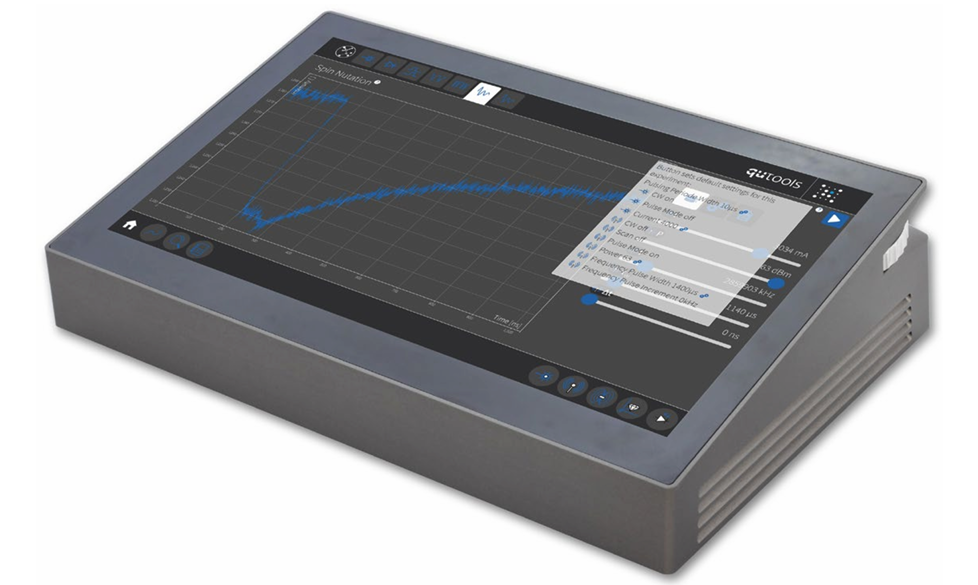
\includegraphics[width=0.65\textwidth]{gfx/diagrams/quEDU.png}
	\caption{\acs{quEDU} \cite{quEDU}}
	\label{fig:4.1}
\end{figure}


Moreover, the \acs{quEDU}, along with its experiment boards, integrates the latest advancements in quantum optics technology to provide an accessible system for academic, research, and applied purposes with remarkable precision. Furthermore, advanced models tailored for scientific applications are also available, delivering exceptional performance to meet the demands of cutting-edge physics experiments.

The qutools Quantum Education kit is specifically tailored for educators, offering a user-friendly and dependable solution to elucidate the intricate concepts of quantum mechanics. This is achieved through the generation and analysis of polarization-entangled photon pairs, as well as the manipulation of electron spins in a diamond.

\section{\acs{quEDU} Key Features}

The \acs{quEDU} system from qutools GmbH offers a highly modular and user-friendly platform designed for hands-on exploration of quantum phenomena. Its versatility allows users to conduct a variety of quantum experiments with ease, making it an ideal tool for both educational and research purposes. Below is a summary of its key features and specific applications:

\begin{itemize}
	\item \textbf{Hands-on Study of Quantum Entanglement: }
	The \acs{quEDU} system enables practical experimentation with quantum entanglement, providing an intuitive platform for users to explore the core concepts of quantum mechanics.
		
	\item \textbf{User-Friendly Operation and Complete System}
	Designed for ease of use, the system features a touchscreen interface and rotary buttons for intuitive control. It is equipped with all necessary components for a complete experimental setup, minimizing the need for additional hardware.
	
	\item \textbf{Expandability with Add-ons}
	To further extend its capabilities, \acs{quEDU} offers add-ons that allow users to expand their experimental scope, making it a versatile tool that grows with the user's needs.
	
	\item \textbf{Specific Applications}
	
	\begin{itemize}
		\item [$\rightarrow$] \textbf{Student Lab Course Experiments: }
		Ideal for educational settings, \acs{quEDU} provides students with hands-on experience in quantum mechanics.
		
		\item [$\rightarrow$] \textbf{Violating Bell's Inequalities: }
		 The system supports experiments that demonstrate the violation of Bell’s inequalities, a key concept in proving the non-classical nature of quantum mechanics.
		 
		 \item[$\rightarrow$] \textbf{NV Center Spin Manipulation: }
		 The system allows for experiments involving NV centers (Nitrogen Vacancy centers in diamond) for spin manipulation, often used in quantum sensing and quantum memory applications.
		 
		 \item [$\rightarrow$] \textbf{Optically Detected Magnetic Resonance(ODMR): }
		 It also supports \acs{ODMR} experiments, which are essential for studying the properties of quantum systems under different magnetic fields.
		 
	\end{itemize}
	
	\item \textbf{Control and Usage}
	\begin{itemize}
		\item [$\rightarrow$] \textbf{TouchScreen and Rotary Buttons: }
		Easy control through an intuitive interface.
		
		\item [$\rightarrow$] \textbf{6 Ports for Experiment Boards: }
		Flexible connections to accommodate various experimental modules.
		
		\item [$\rightarrow$] \textbf{Remote Desktop via WLAN, Ethernet: }
		The system can be accessed remotely, allowing for convenient control and monitoring through WLAN or Ethernet connections.
		
	\end{itemize}
	
	\item \textbf{Detection and Analysis}
	\begin{itemize}
		\item [$\rightarrow$] \textbf{4 Temperature - Controlled APDs: }
		The system includes Avalanche Photodiodes (APDs) with fiber ports for precise photon detection, featuring temperature control to ensure stability during measurements.
		
		\item [$\rightarrow$] \textbf{Time tagging Electronics: }
		Equipped with time tagging electronics with picosecond precision, enabling accurate measurement of time-correlated photon events.
		
		\item[$\rightarrow$] \textbf{Singles and Coincidence Counting: }
		 Provides the ability to count both single and coincidence photon events, crucial for many quantum experiments.
		 
		 \item[$\rightarrow$] \textbf{Analysis and Data Processing: }
		  Includes tools for analyzing and processing measurement data, streamlining the workflow from experiment to result interpretation.
	
	\end{itemize}
\end{itemize}

\section{quNV - Nitrogen Vacancy Center Board}

The \acs{NV} experiment board provides an opportunity to explore the characteristics of nitrogen vacancy centers in diamond. This includes the examination of \acs{NV} center fluorescence, the manipulation of electron spins, the application of optically detected magnetic resonance, and the sensing of magnetic fields in samples.

\begin{itemize}
	\item [$\rightarrow$] \textbf{Setup with \acs{quEDU}: }
	The board must initially be connected to the \acs{quEDU} using a DisplayPort cable, which serves both as a power supply and for data communication. Two optical fibers link the \acs{NV} center board to the avalanche photodiodes (APDs) of the \acs{quEDU}. One of these fibers is responsible for collecting the red fluorescence emitted by the \acs{NV} center through the objective, subsequently transmitting it to one of the APDs. The second fiber is utilized to convey a portion of the green excitation light, facilitating closed-loop control of the laser.
	
	\begin{figure}[htbp]
		\centering
		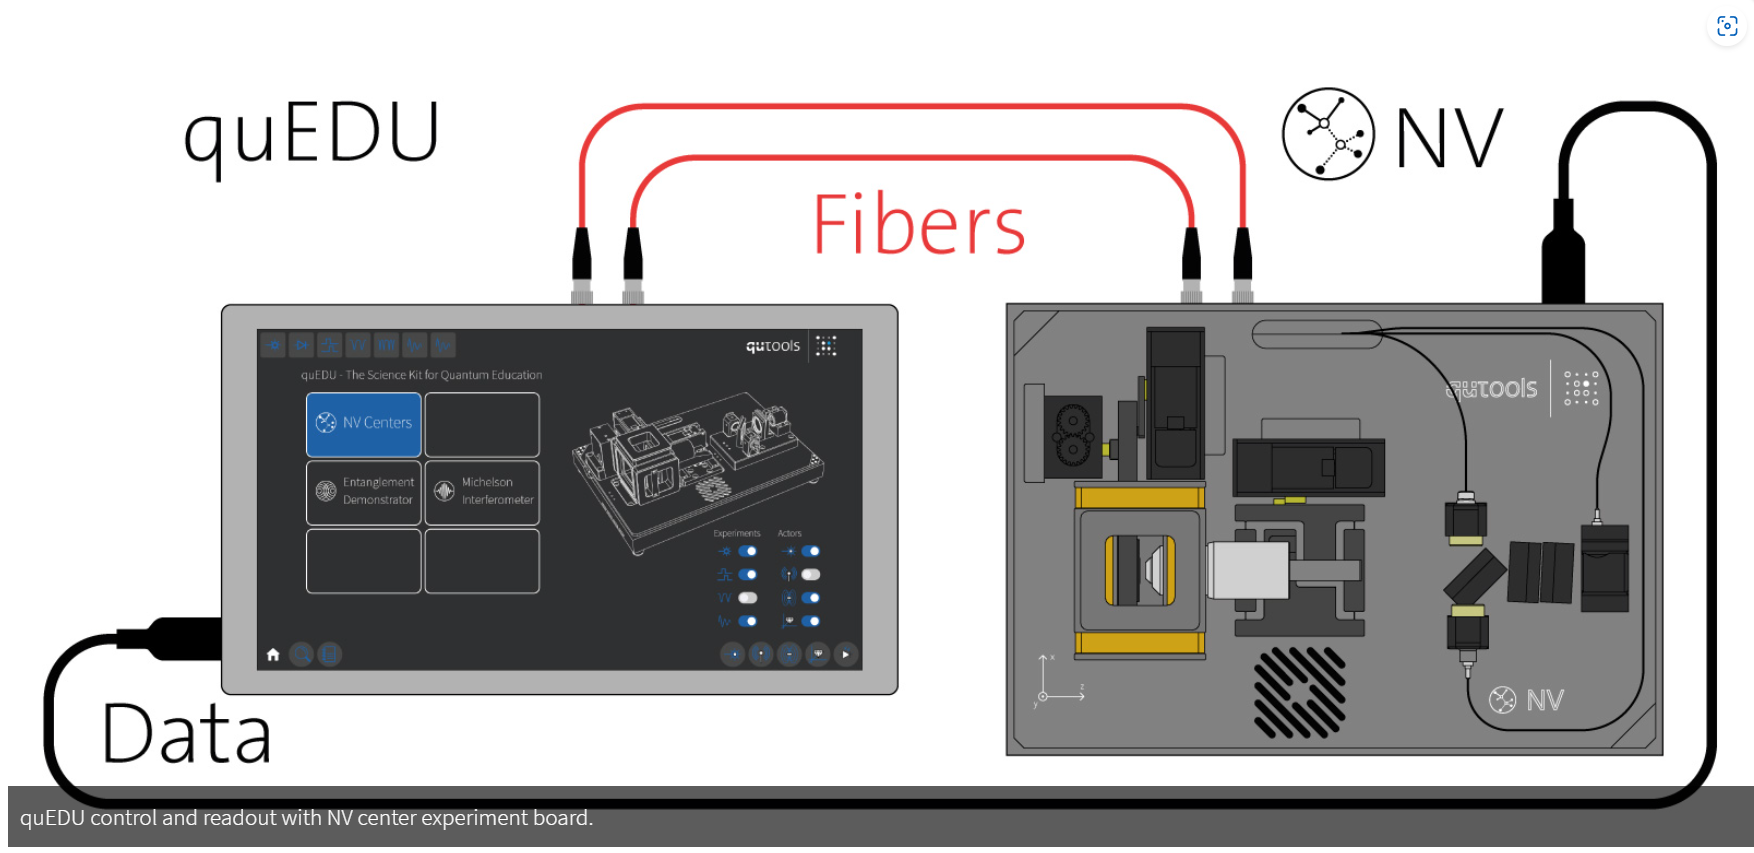
\includegraphics[width=0.50\textwidth]{gfx/diagrams/quNV_quEDU.png}
		\caption{The \acs{quEDU} manages all experiments and gauges their photon output, while an \acs{NV} board explores nitrogen vacancy centers in diamond.\cite{quNV_quEDU}} 
		\label{fig:4.2}
	\end{figure}
	
	\begin{figure}[htbp]
		\centering
		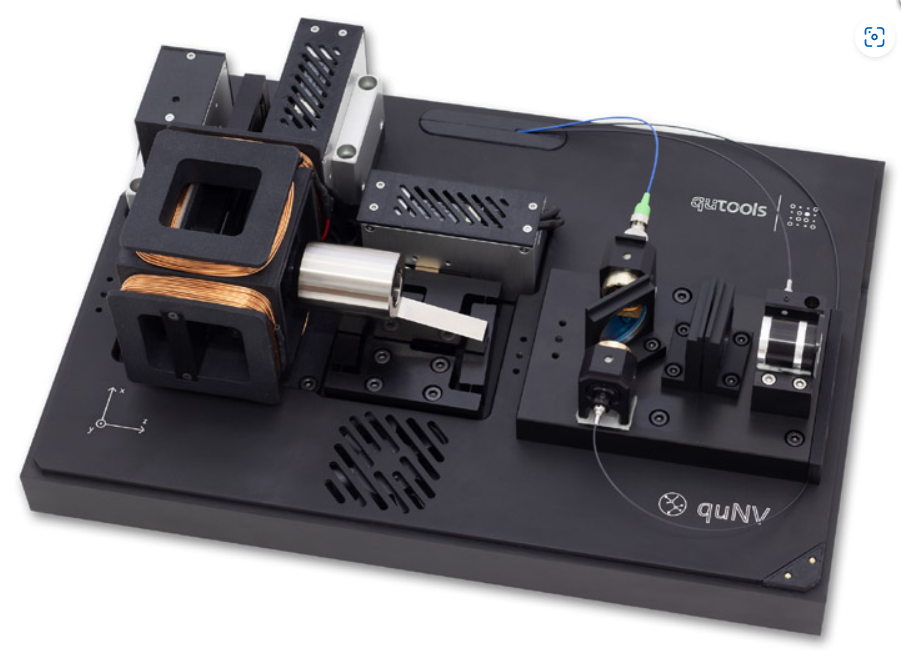
\includegraphics[width=0.40\textwidth]{gfx/diagrams/quNV.png}
		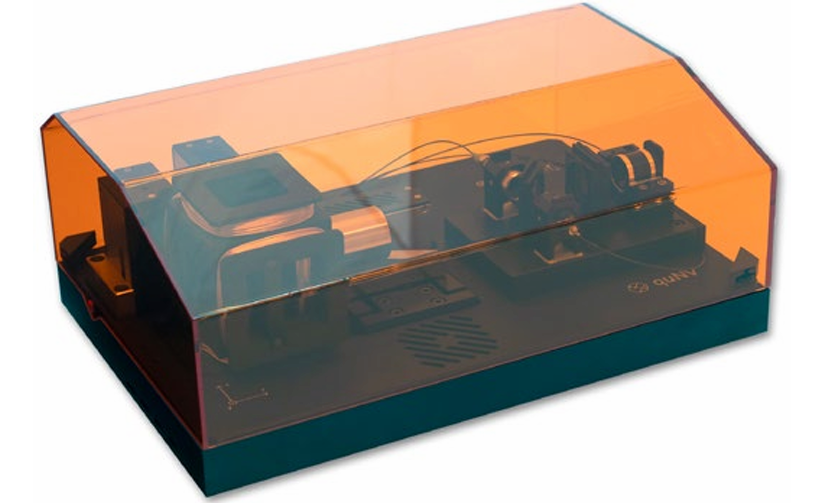
\includegraphics[width=0.40\textwidth]{gfx/diagrams/quNV_interlock.png}
		\caption{\acs{quNV}\cite{quNV}} 
		\label{fig:4.3}
	\end{figure}
	
	\item[$\rightarrow$] \textbf{Laser and Sample Alignment: }
	The subsequent task involves the precise alignment of the diamond in front of the microscope objective. We commence by activating the powerful green laser located beneath the orange safety cover. Utilizing the alignment controls available in the graphical user interface, we can adjust the sample's position to ensure it is perpendicular to the direction of the laser beam. Ultimately, we observe the red fluorescence emitted by the nitrogen-vacancy (NV) center through the safety glass. Fine alignment in all three dimensions is achieved by plotting the data obtained from the avalanche photodiode (APD) on the \acs{quEDU} screen. \clearpage
	
	% Add vertical space between figures	
	\vspace{2cm}  % Adjust the value to the desired amount of space
	
	\begin{figure}[htbp]
		\centering
		\includegraphics[width=0.75\textwidth]{gfx/diagrams/green_Laser_intensity.png}
		\caption{The intensity of the green laser has been measured using Avalanche Photo Diodes (APDs). The recorded spikes indicate that the laser is operating in sequencer mode, characterized by bursts of laser pulses. Conversely, the steady portion reflects the laser's operation in continuous mode, where it remains consistently activated. } 
		\label{fig:4.4}
	\end{figure}
	
	% Add vertical space between figures
	\vspace{1cm}  % Adjust the value to the desired amount of space
	
	\begin{figure}[H]
		\centering
		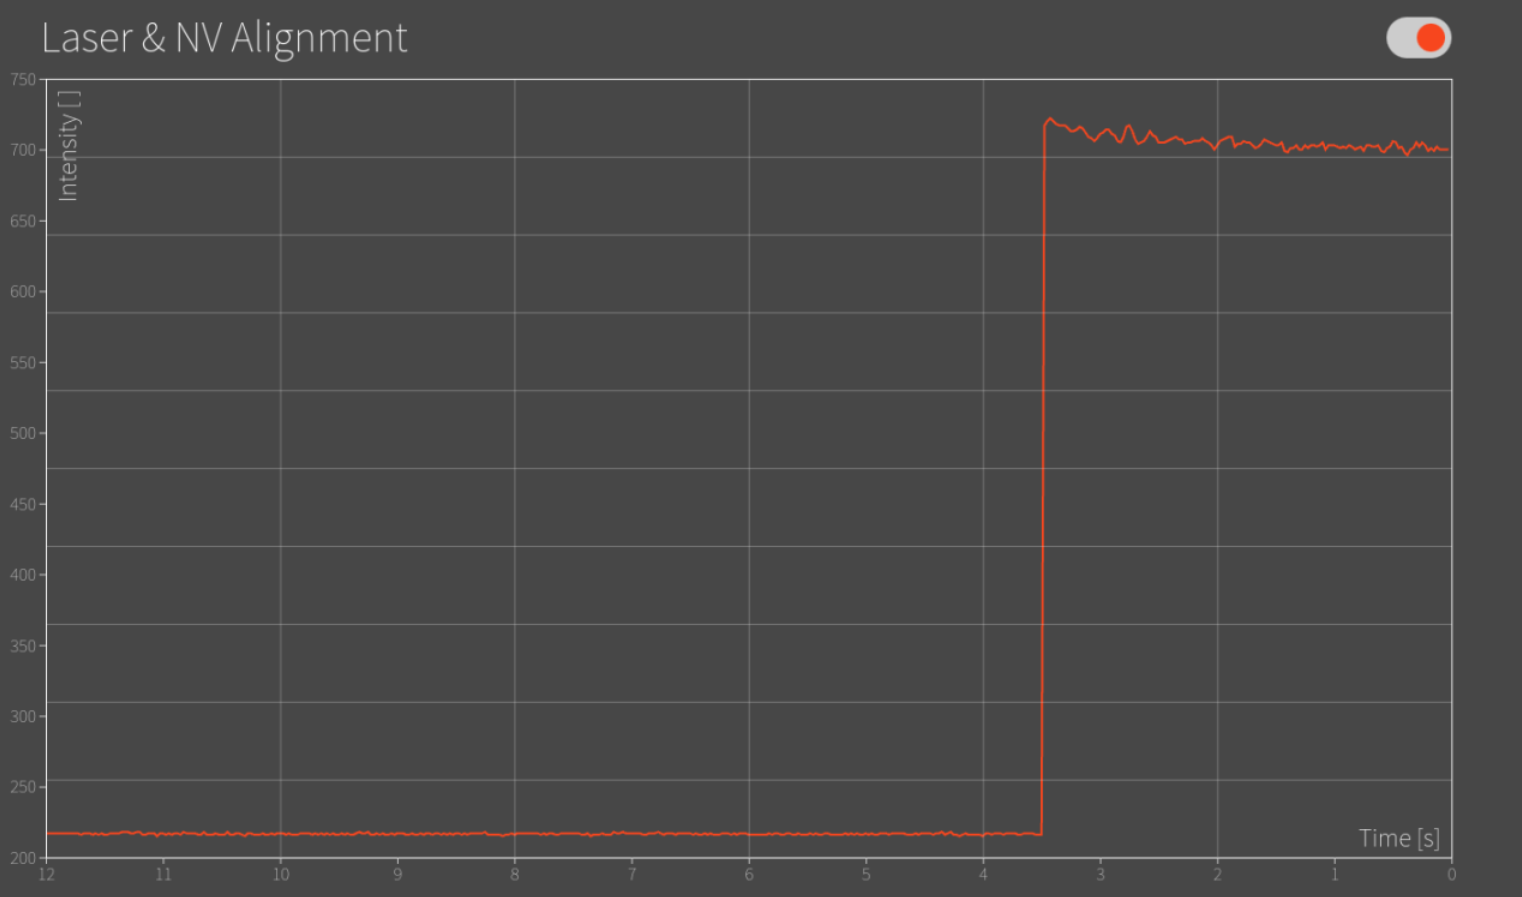
\includegraphics[width=0.75\textwidth]{gfx/diagrams/Red_floursence_from_diamond.png}
		\caption{This image illustrates the red fluorescence emitted from the diamond as a result of the interaction between the incoming green laser and the diamond.} 
		\label{fig:4.5}
	\end{figure} \clearpage
	
	
	\item[$\rightarrow$] \textbf{ODMR Scan: }
	To initiate an ODMR (optically detected magnetic resonance) scan focused on studying the resonance frequencies, it is essential to achieve a high fluorescence intensity. The process involves activating the microwave source, systematically scanning its frequency, and subsequently plotting the resulting fluorescence data. This procedure typically reveals at least two distinctive dips in the observed fluorescence spectrum. Furthermore, by applying a magnetic field through the coils, we can induce a further splitting of the resonance peaks, a phenomenon known as Zeeman splitting.

	\begin{figure}[H]
		\centering
		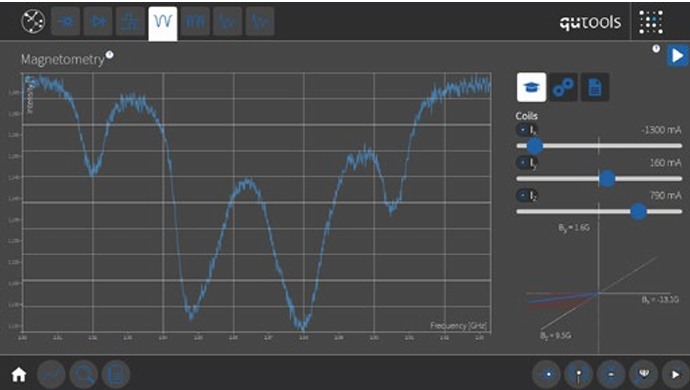
\includegraphics[width=0.75\textwidth]{gfx/diagrams/ODMR.png}
		\caption{The GUI controls the coils to create a 3D magnetic field, while a microwave frequency sweep captures the ODMR spectra of the diamond.\cite{quEDU}} 
		\label{fig:4.6}
	\end{figure}
	
		
\end{itemize}

\section{Software Architecture of quEDU-NV Python Software}

The \acs{quEDU} Python software is developed to manage quantum experiments by leveraging the qudi framework. qudi’s architecture promotes modular design, making it well-suited for complex scientific applications by enforcing clear separation between components. This enables better maintainability and easier scaling for a variety of quantum experiment setups. The core of the \acs{quEDU} system adopts qudi’s structural model, which centers on three primary components: the \acs{GUI}, Logic, and Hardware modules.

\begin{figure}[H]
	\centering
	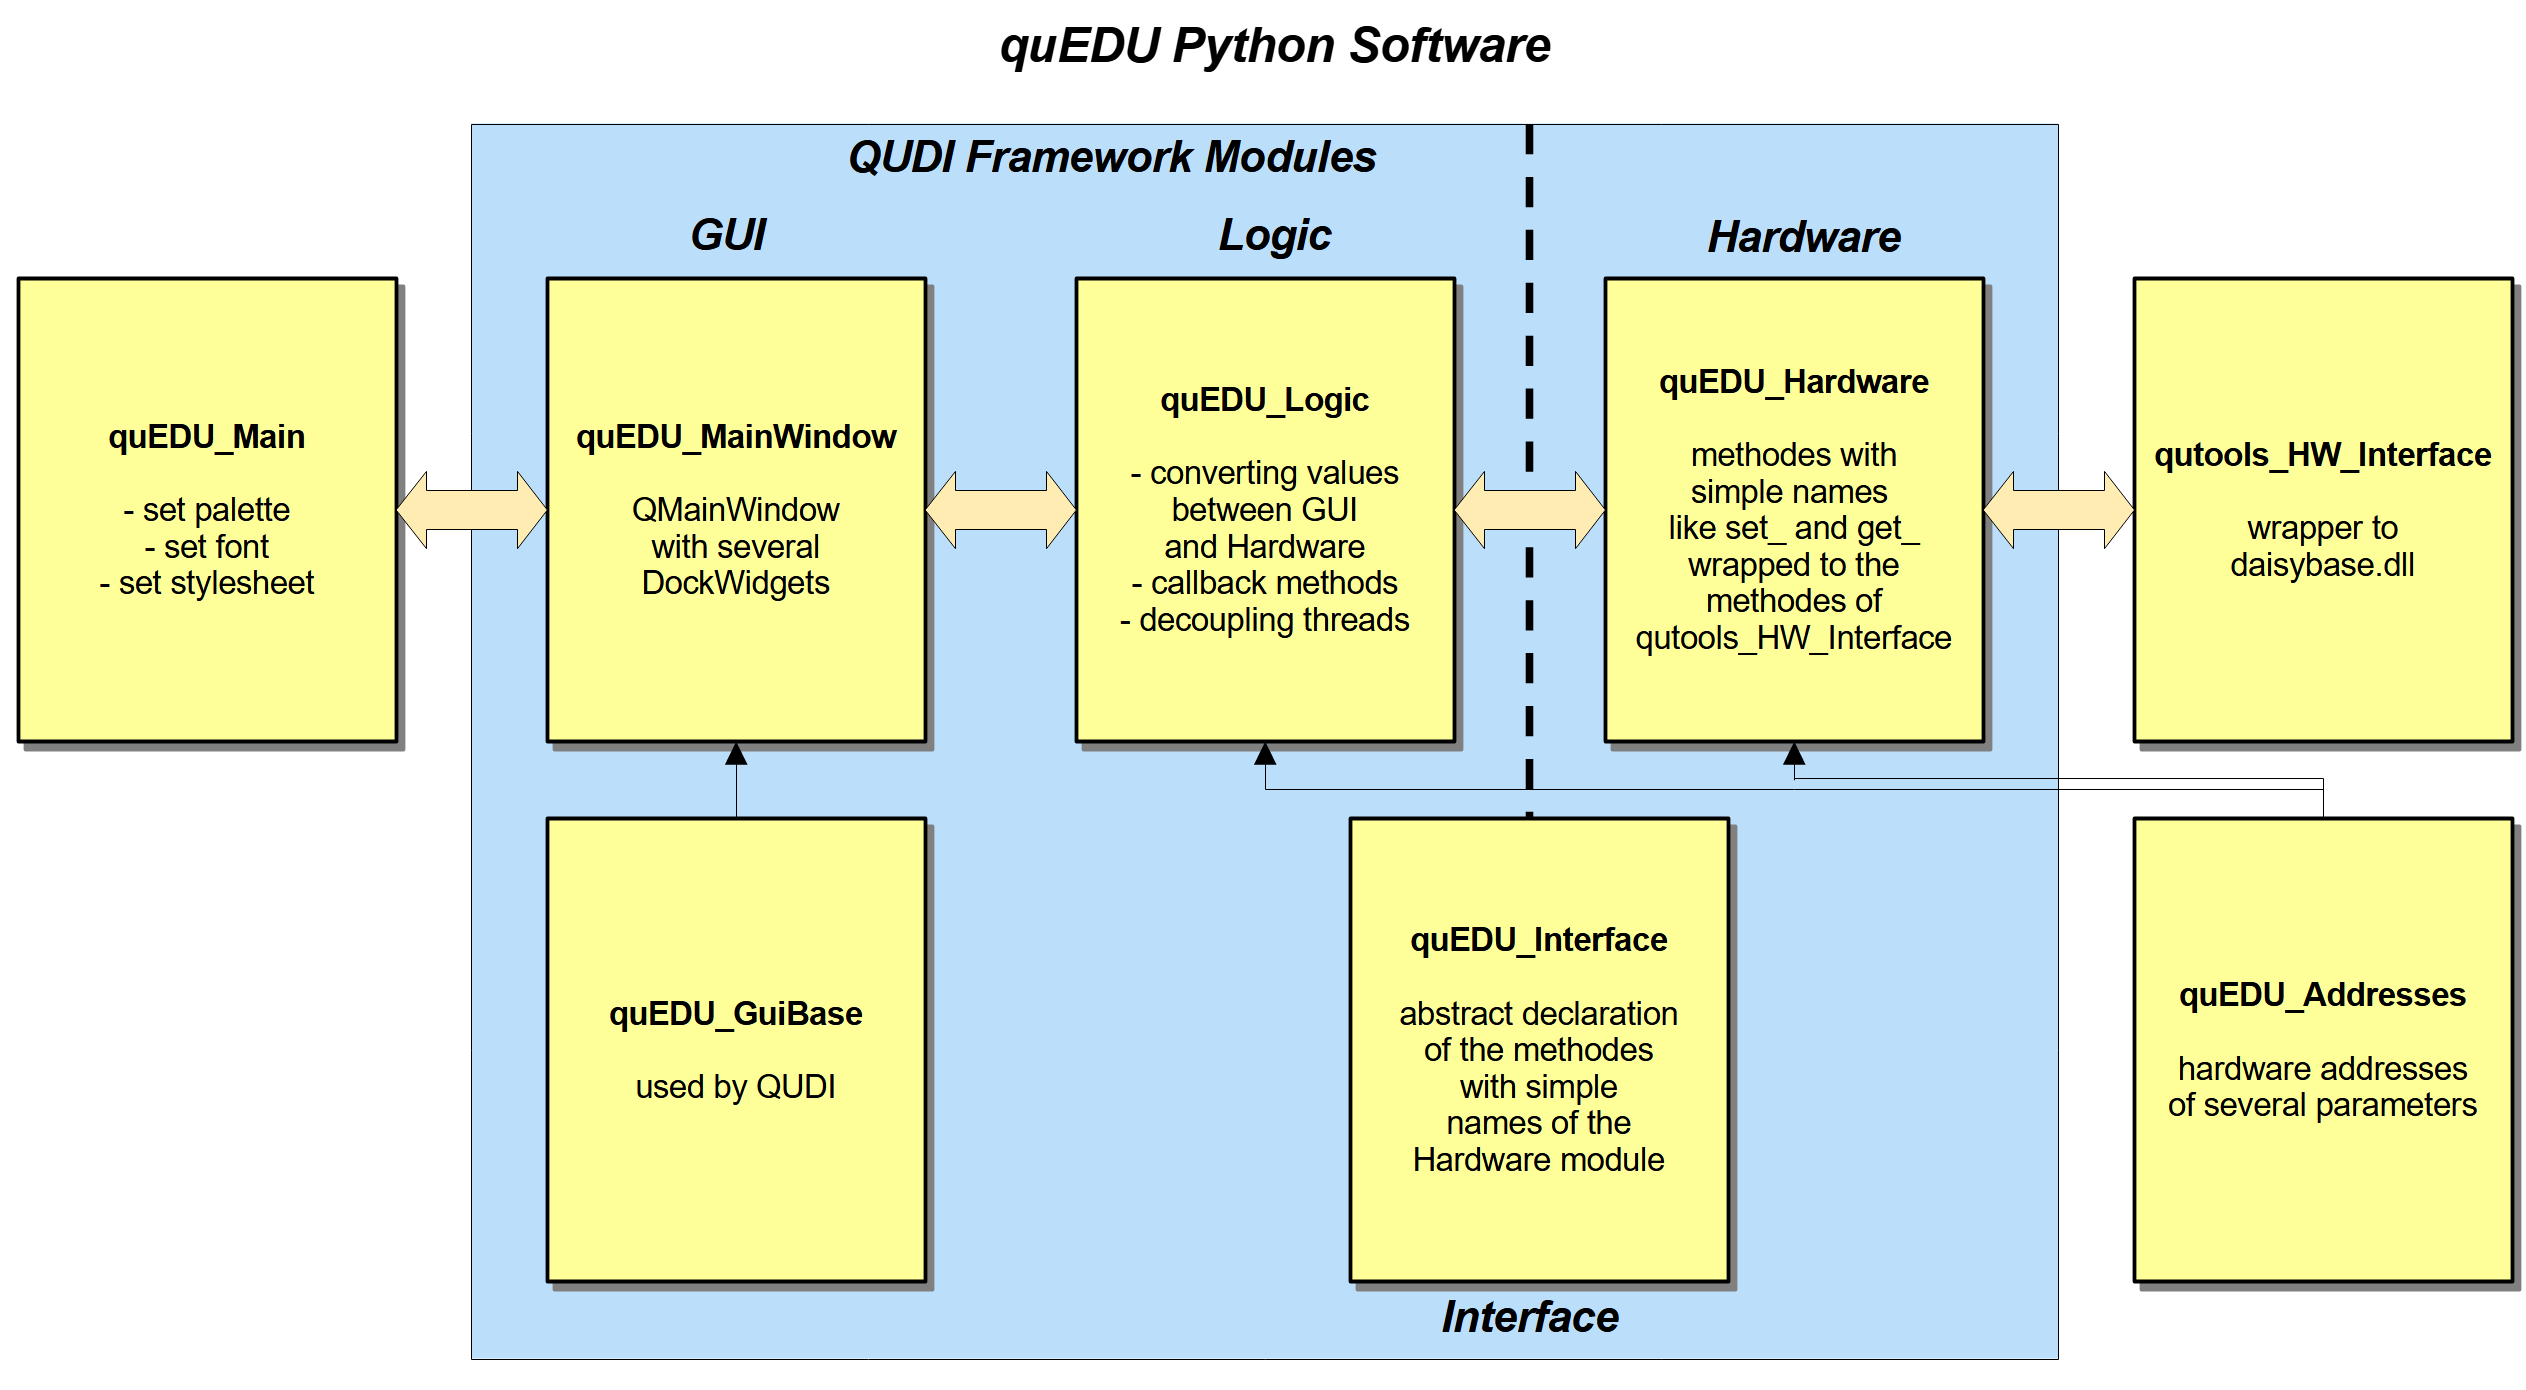
\includegraphics[width=1.0\textwidth]{gfx/diagrams/quEDU_NV_Python_GUI_Software_Block_Diagram.png}
	\caption{quEDU/NV Python Software Block Diagram} 
	\label{fig:4.7}
\end{figure}

\begin{itemize}
	\item \textbf{GUI (Graphical User Interface) Module: } This component handles the graphical elements and user interactions, enabling intuitive access to experimental controls and data displays.
	\item \textbf{Logic Module: } Handles the core functionality and the business logic, coordinating data processing and management.
	\item \textbf{Hardware Module: } Interfaces directly with quantum experiment hardware via the qutools\_HW\_Interface.py wrapper, which accesses the qutools daisybase.dll.
\end{itemize}

The GUI module provides interactive widgets for user input, while the Logic module performs calculations or manipulations based on user inputs. The Hardware module acts as the bridge between the software and the experimental hardware, enabling direct communication with hardware elements.

\subsection{Standalone Operation Without qudi}

When running independently of qudi, the \acs{quEDU} software utilizes a main module, quEDU\_Main.py, which serves as the entry point to start the application. This main module initializes each component separately and launches the software.

In the absence of qudi, all modules connect directly, potentially resulting in a tightly coupled structure. This could cause issues in a standalone environment, as all modules would be operating in a single thread, with both Logic and Hardware operations potentially blocking the GUI and impacting responsiveness. To mitigate this, qudi introduces a unique architectural feature for linking modules and managing communication effectively.

\subsection{qudi’s Connector Class for Decoupling and Multithreading}

One of the key architectural elements of qudi is the connector class, which decouples modules by avoiding direct imports. Instead, module connections are configured through the quEDU.cfg file, allowing qudi to dynamically link them at runtime.

qudi also separates modules into different threads, preventing the Logic and Hardware components from blocking the GUI thread. This multithreading ensures a responsive interface, even when complex hardware or logic operations are active.

\subsection{Signal-Slot Mechanism Using PySide2}

qudi leverages Python Qt modules, specifically PySide2, to facilitate communication between modules. PySide2, a Python binding of the Qt framework, provides a powerful signal-slot mechanism for inter-module communication that fits naturally into qudi’s architecture.

In the signal-slot pattern, different components communicate through signals (events) and slots (reactions), allowing an event in one module to trigger a response in another. This design enables efficient, asynchronous communication between the GUI and Logic modules, contributing to both decoupling and responsiveness.

\begin{itemize}
	\item \textbf{Signal Transmission: }
	The GUI module consists of various interactive widgets, such as buttons, sliders, and text fields. Each widget can emit signals in response to user actions, such as editing.finished, button.clicked, or slider.moved. When a user interacts with a widget, it sends out a signal containing the current value or state. This signal is directed to the Logic module, where it might trigger further processing or a value conversion, depending on the type of action performed.
	
	\item \textbf{Logic to \acs{GUI} Communication: }
	After processing the input, the Logic module may send updated values or responses back to the GUI. This is done through additional signals emitted by the Logic module. For instance, if a certain computation is triggered in the Logic module due to a user action, the result is then packaged in a signal and sent back to the GUI, where the corresponding slots in the GUI widgets receive the values and update the interface. This bidirectional communication flow allows the user interface to reflect real-time changes based on interactions with the underlying Logic module.
	
\end{itemize}

The installation process for the qudi Python framework is detailed in the Appendix \ref{appendixB: qudi_installation}

\section{quEDU-NV Python Graphical User Interface Design}

The \acs{quEDU} platform serves as a sophisticated tool for conducting a variety of quantum physics experiments. It contains single photon detectors and time tagging electronics for data acquisition and analysis as well as digital interfaces to control the experiments. The \acs{quEDU} and its experiment boards combine the latest achievements in quantum optics technology into easy-to-use system for academic, research and applied purposes with high precision.

The \acs{NV} experiment board allows users to experience the various properties of nitrogen vacancy centers in diamond, as previously detailed in this report.  At the heart of the \acs{NV} is a green laser focused on the nitrogen-doped diamond through a microscopic objective. The diamond begins to fluoresce in the red wavelength range. This light is collected by the objective and, after some filtering, is coupled into a fiber. The fiber is connected to the \acs{quEDU} and the florescence can be analyzed. 

The diamond sample itself is in close proximity to a microwave antenna and is surrounded coils producing a user defined homogeneous magnetic field. In addition, the \acs{quEDU}s included pattern generator is precisely controlling pulse sequences for laser, microwave, and readout, enabling a multitude of spin-control experiments. 

This section delineates the final Python graphical user interface (GUI) developed for the quEDU-NV devices within the qudi framework.  The \acs{GUI} has a toolbar and menu sections to navigate through different experiments.

\subsection{Home Screen}

\begin{figure}[htbp]
	\centering
	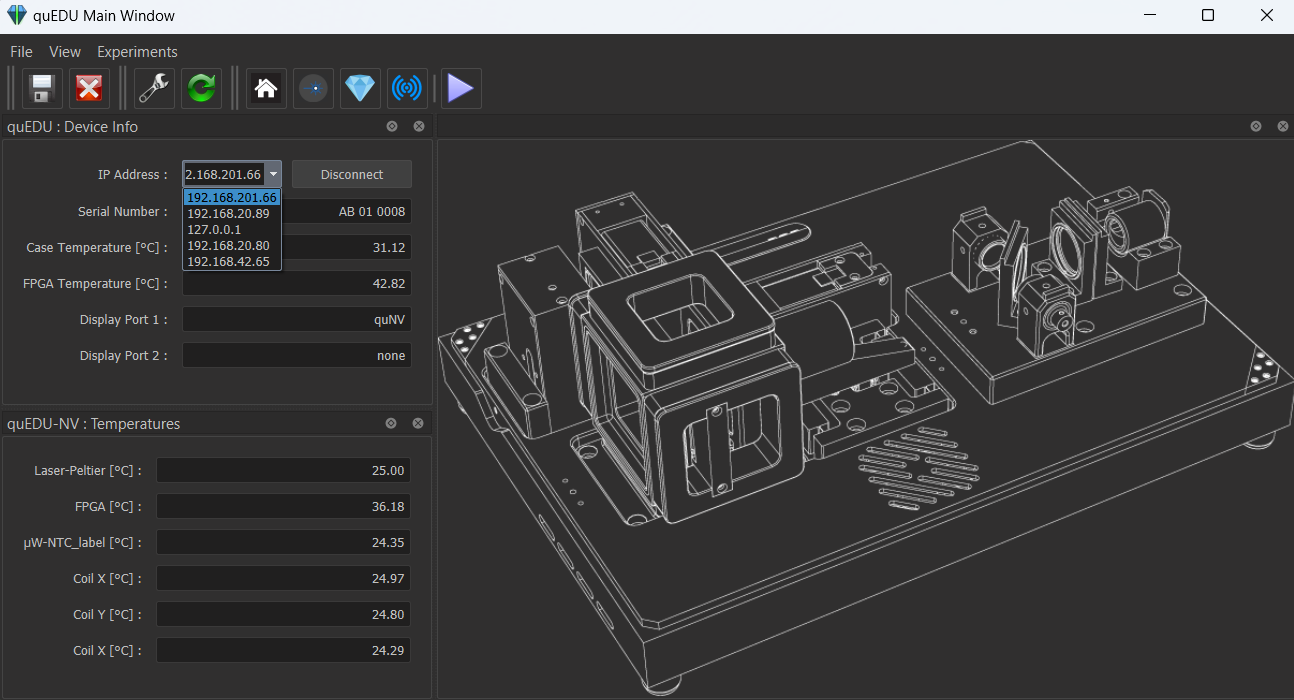
\includegraphics[width=1.0\textwidth]{gfx/diagrams/quEDU_GUI_Home.png}
	\caption{Home Screen} 
	\label{fig:4.8}
\end{figure}

The homepage provides essential device information for the connected \acs{quEDU} system. Connection to the device is established through Ethernet, and the application retains IP addresses for streamlined future connections. The Device Info dockwidget shows key details, such as the serial number of the connected \acs{quEDU} device and current temperature readings. It also indicates if additional devices are connected to the \acs{quEDU}. In this setup, the application is designed for quEDU-NV, with the \acs{quNV} add-on linked to the main system. Additionally, the quEDU-NV Temperatures dockwidget displays temperature data for various electronic and mechanical components within the \acs{quNV} setup. Additionally, the dockwidgets offer a flexible interface: they can be repositioned across the screen to suit user preferences. Users can also remove or view specific dockwidgets as needed, allowing them to focus on the most relevant information.

\subsection{Laser properties}

This section presents the Laser controls for the \acs{quNV} device. The intensity plot serves as a visual representation of the laser intensity.

\begin{figure}[htbp]
	\centering
	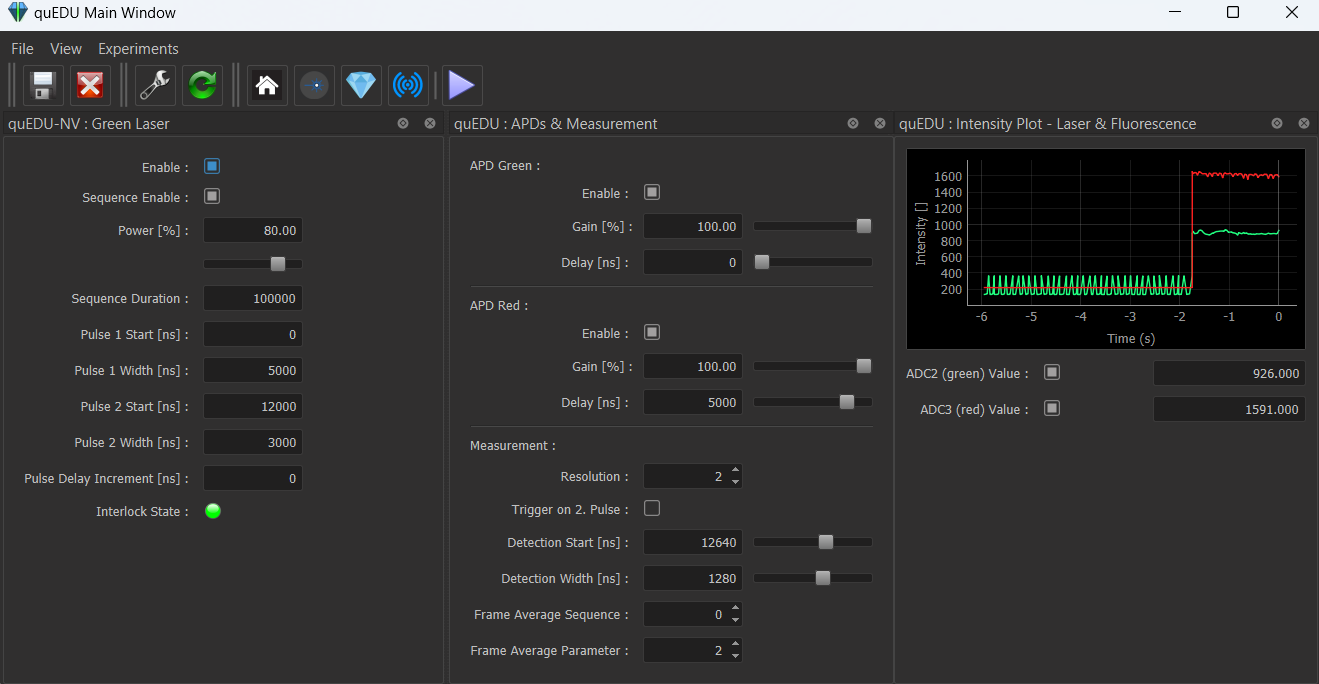
\includegraphics[width=1.0\textwidth]{gfx/diagrams/Laser_Properties.png}
	\caption{Laser Properties} 
	\label{fig:4.9}
\end{figure}

The Green Laser dockwidget facilitates the adjustment of the laser's operational mode, allowing it to be configured for either continuous mode or Sequence/Pulse mode. The accompanying laser intensity plot illustrates the transition of the green laser—from Sequence/Pulse mode to continuous mode. The red plot represents the fluorescence captured by the avalanche photodiodes (APDs) when the green laser interacts with a diamond situated at the heart of \acs{quNV}. This interaction results in the emission of red fluorescence from the diamond upon exposure to the green laser.

The \acs{APD}s \& Measurement section allows us to manage the \acs{APD}s effectively. Here, we can enable or disable specific \acs{APD}s based on whether we want to view their intensity on the plot. Additionally, adjusting the gain of an \acs{APD} will impact its intensity.

\subsection{Confocal Alignment}

When the green laser interacts with the nitrogen-doped diamond, it produces a high-intensity red fluorescence. In the \acs{quNV} setup, motors control the movement of the microscopic objective, which emits the green laser. This objective scans along the x, y, and z axes to locate three distinct diamond particles. This precise positioning is essential for further analysis of the \acs{NV} centers' properties within the diamond.

There are predefined limits established within the server/\acs{FPGA} that dictate the movement range of the motors. These limits are illustrated by the red rectangle on the XY-image plot. The blue rectangle represents the "Region of Interest," indicating the area where the motors conduct their scanning. Notably, when there is a high intensity (represented as red, grey, or blue based on the selected color), the corresponding pixel will appear vividly bright on the XY-image plot, thereby indicating the presence of a diamond.

The Motion Control and Diamond Scan dock widgets facilitate the maneuvering of the motors. The Motion Control dock widget presents the current positions of the motors, while also allowing users to specify target positions. A red cursor in the shape of a target is displayed on the XY-image plot, indicating the desired position of the motors, which can be established within the Motion Control dock widget. Upon clicking the Start button in the Motion Control dock widget, the green circle cursor on the XY-image plot, representing the current position, will transition to the target position.

\begin{figure}[H]
	\centering
	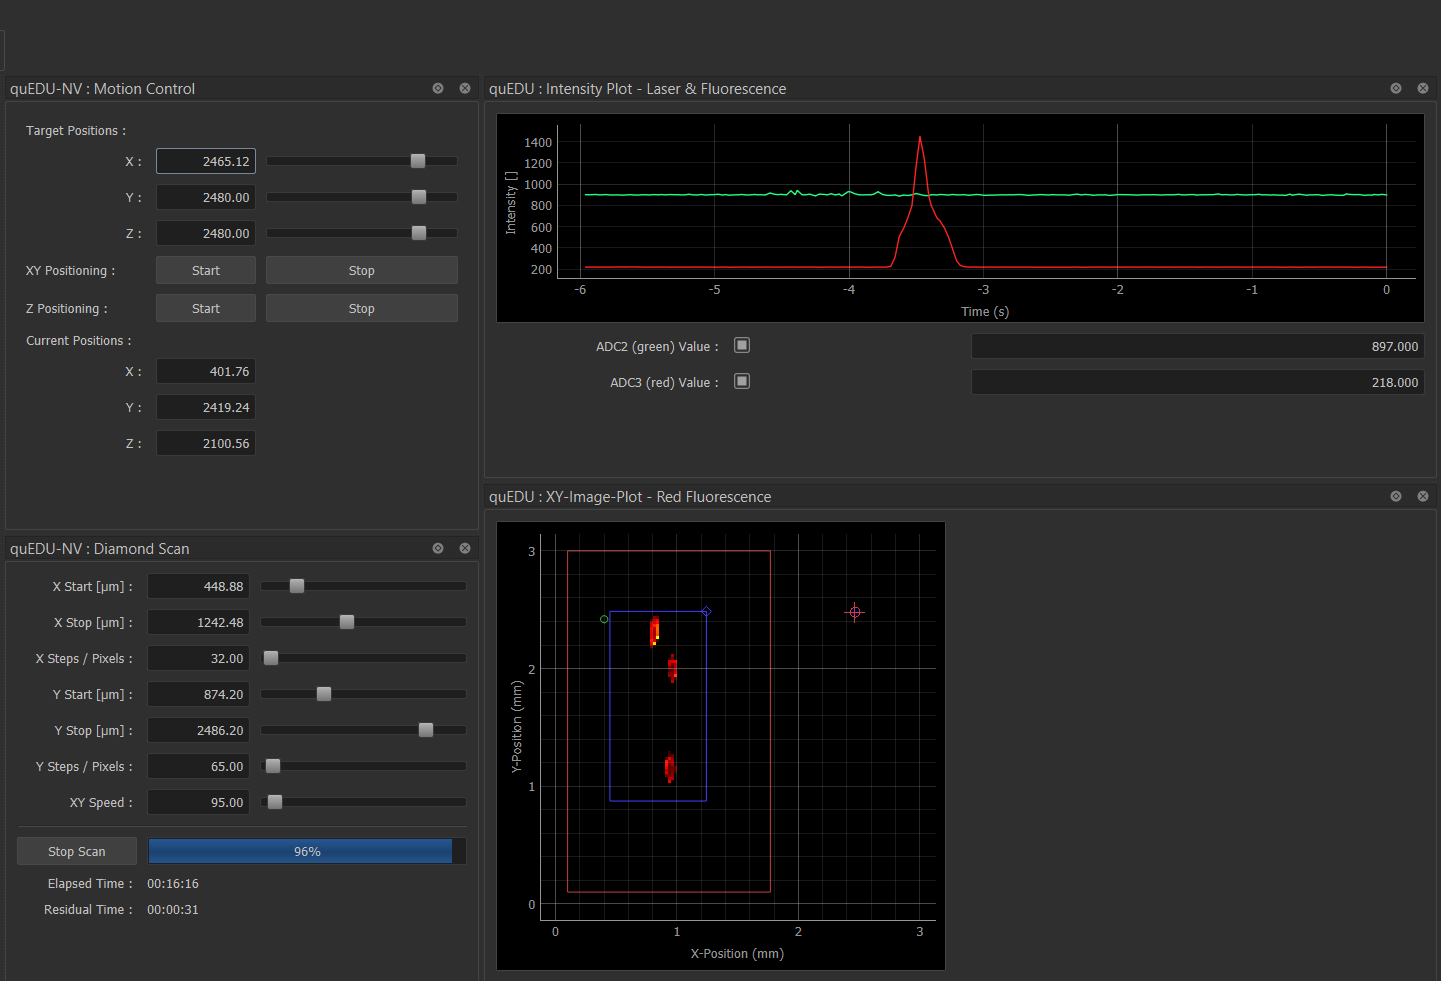
\includegraphics[width=1.0\textwidth]{gfx/diagrams/confocal_alignment.png}
	\caption{Confocal Alignment} 
	\label{fig:4.10}
\end{figure}

The scanning process for locating diamonds can be conducted within the Diamond Scan dock widget. Control over motor movements along the X, Y and Z axes is facilitated, and users have the option to configure the steps or pixels between the initial and final positions. Additionally, this dock widget provides information regarding the total duration of the scan as well as the elapsed time.

The option to designate target positions based on diamond pixels is also available. We can select pixels where a diamond has already been identified from the XY-Image plot, which correspond to regions of higher red fluorescence intensity. This is illustrated in the image below. In the example provided, the red target cursor is positioned on a diamond pixel, and the "start" option has been selected in the Motion Control dock widget. Consequently, the X, Y, and Z coordinates are established for that specific diamond pixel. The elevation in red intensity in the plot further corroborates this observation. \clearpage

\begin{figure}[htbp]
	\centering
	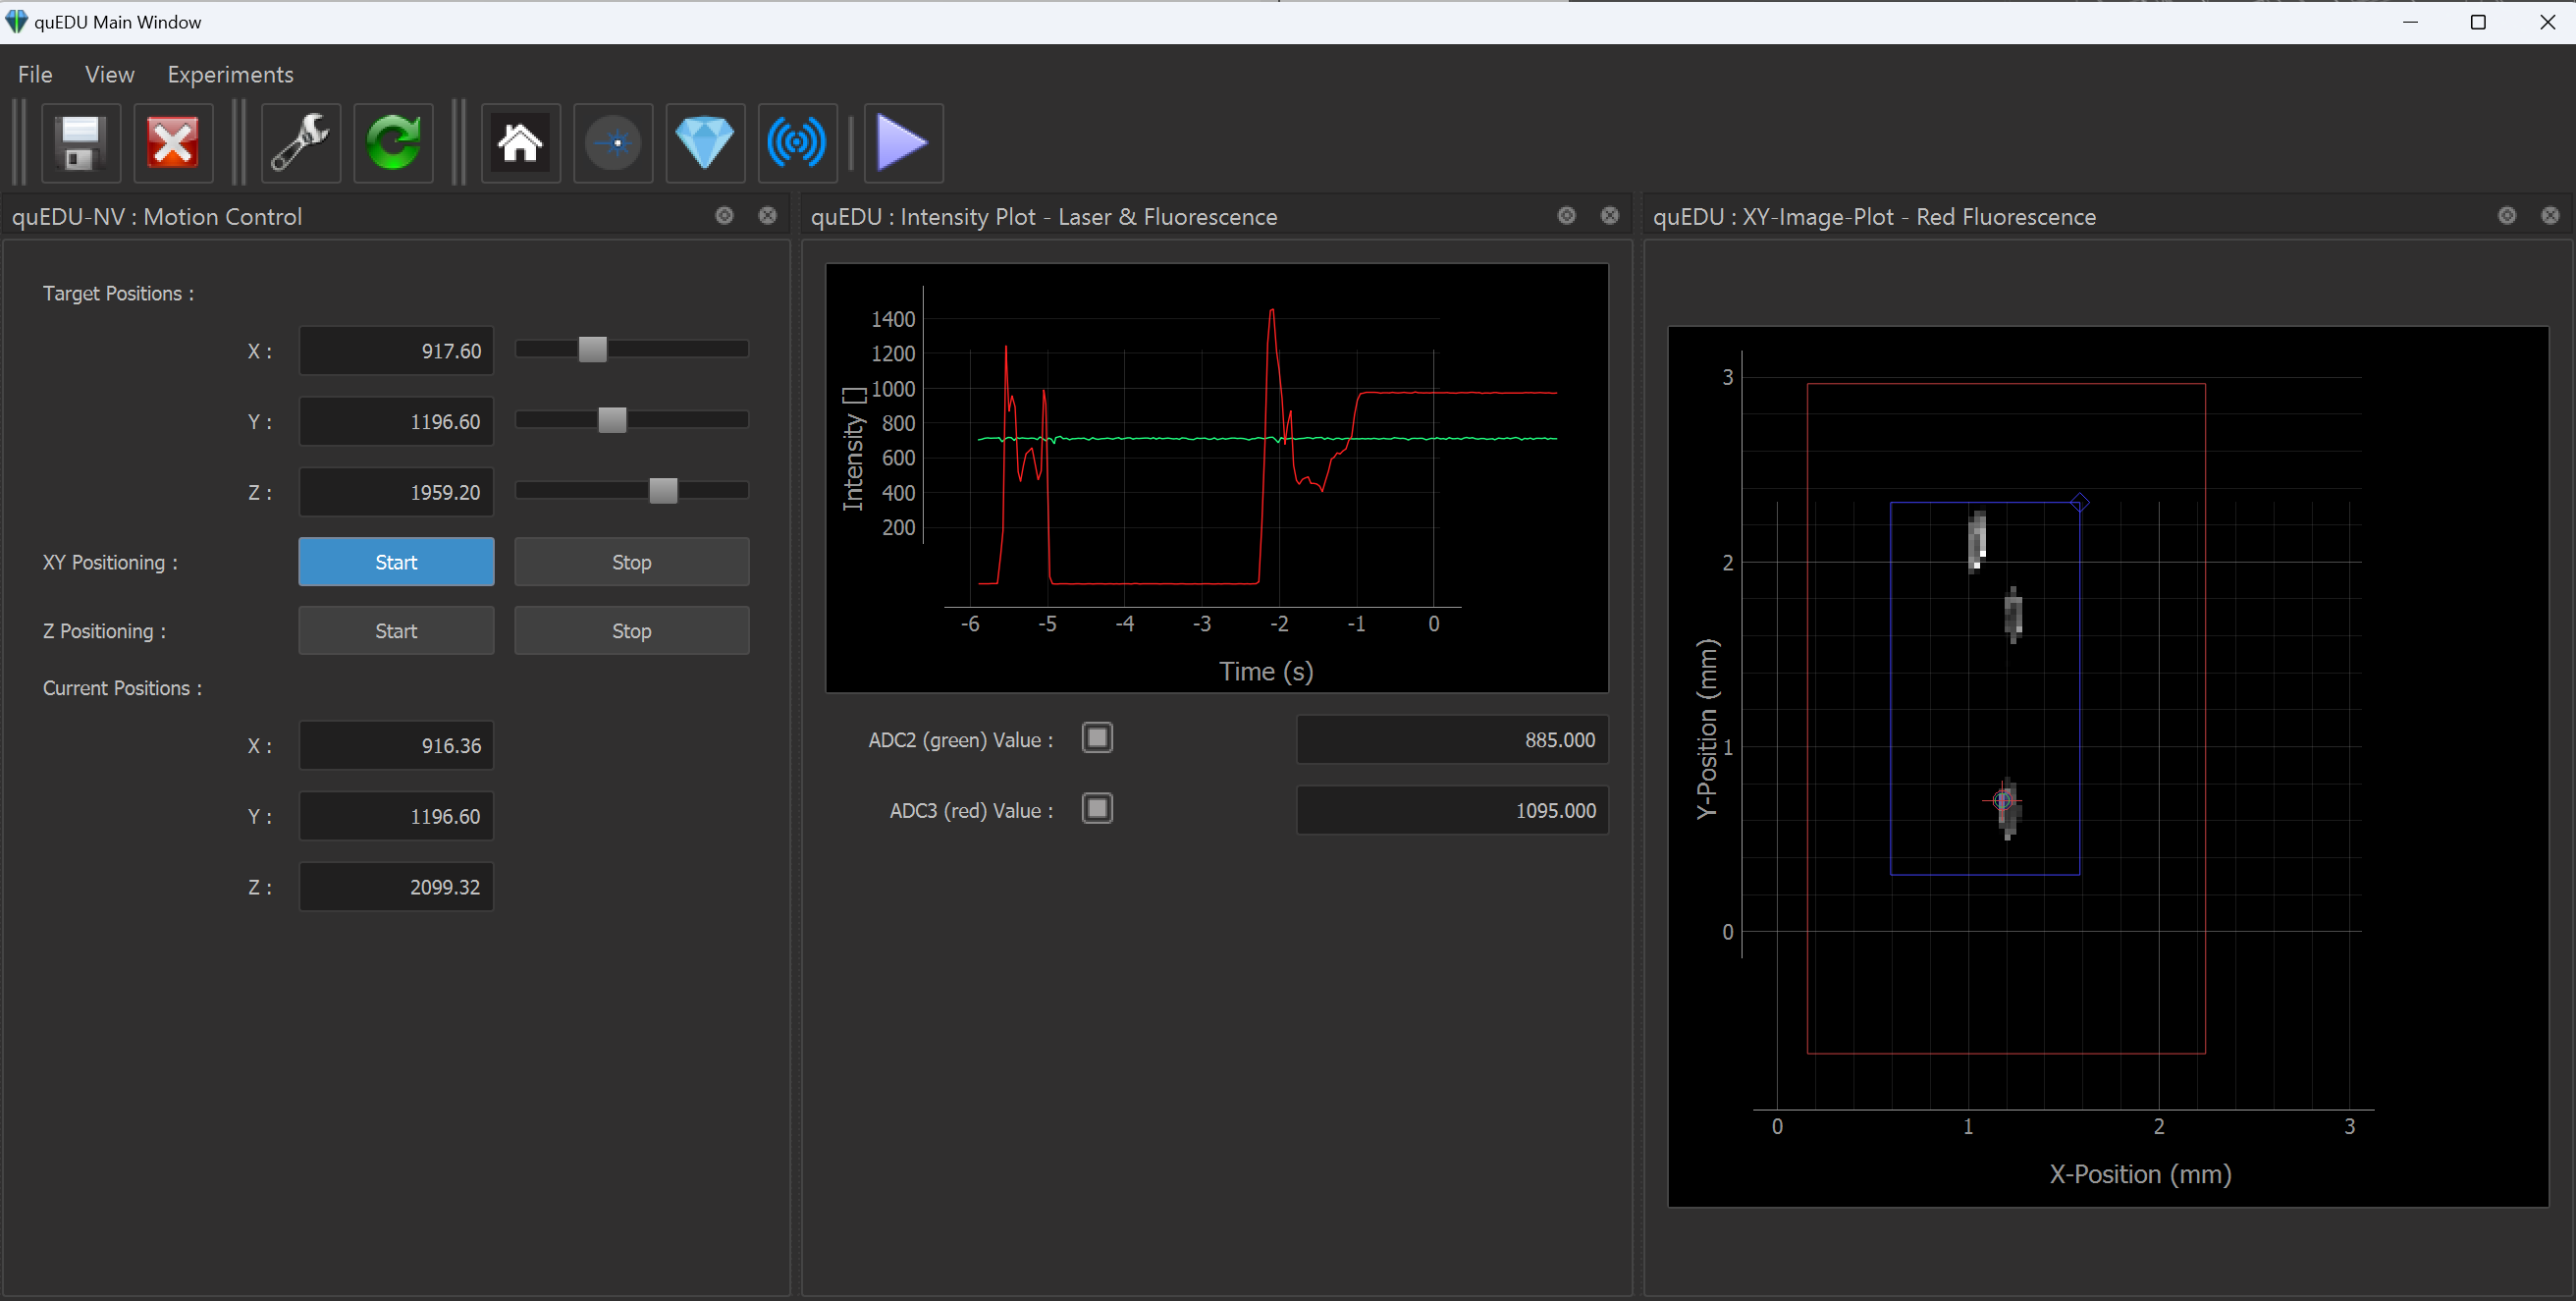
\includegraphics[width=1.0\textwidth]{gfx/diagrams/set_target_pos.png}
	\caption{Target positions are set based on the Diamond identified pixels} 
	\label{fig:4.11}
\end{figure}

\subsection{Optically Detected Magnetic Resonance (ODMR)}

\acs{ODMR} allows users to measure magnetic resonance of NV centers by using a combination of optical and microwave fields. The red florescence from the \acs{quNV} changes depending on the NV center's electronic spin state, simultaneously, when a microwave field is applied to the \acs{NV} centers, and the microwave frequency matches the resonance frequency of the NV center's spin states (typically determined by the local magnetic or electric fields), a drop in red fluorescence intensity is observed.

This fluorescence drop, or "dip," within the \acs{ODMR} spectrum facilitates the identification of the resonance frequency, directly correlating with the strength of the local magnetic field or the accompanying temperature. The resonance frequencies associated with NV centers are notably responsive to variations in magnetic fields and temperature. Therefore, by conducting a thorough analysis of these fluorescence dips, \acs{quNV} systems can adeptly measure environmental parameters with exceptional sensitivity. 

\acs{ODMR} is particularly advantageous in the realm of quantum sensing applications, wherein precise measurements of magnetic fields at the nanoscale are essential, particularly in fields such as materials science, biology, and fundamental physics.

The icon located adjacent to the diamond icon in the toolbar represents the \acs{ODMR} section. Several presets are available concerning \acs{ODMR}. It is imperative that the laser operates in pulse or sequencer mode rather than continuous mode. Additionally, the Pulse Enable option must be activated within the Microwave dock widget. Two plots, namely the Oszi-T and Oszi-P plots, allow for the visualization of the pulse mode of the green laser as well as the \acs{ODMR} spectrum, represented by the dip in red fluorescence.

\begin{figure}[htbp]
	\centering
	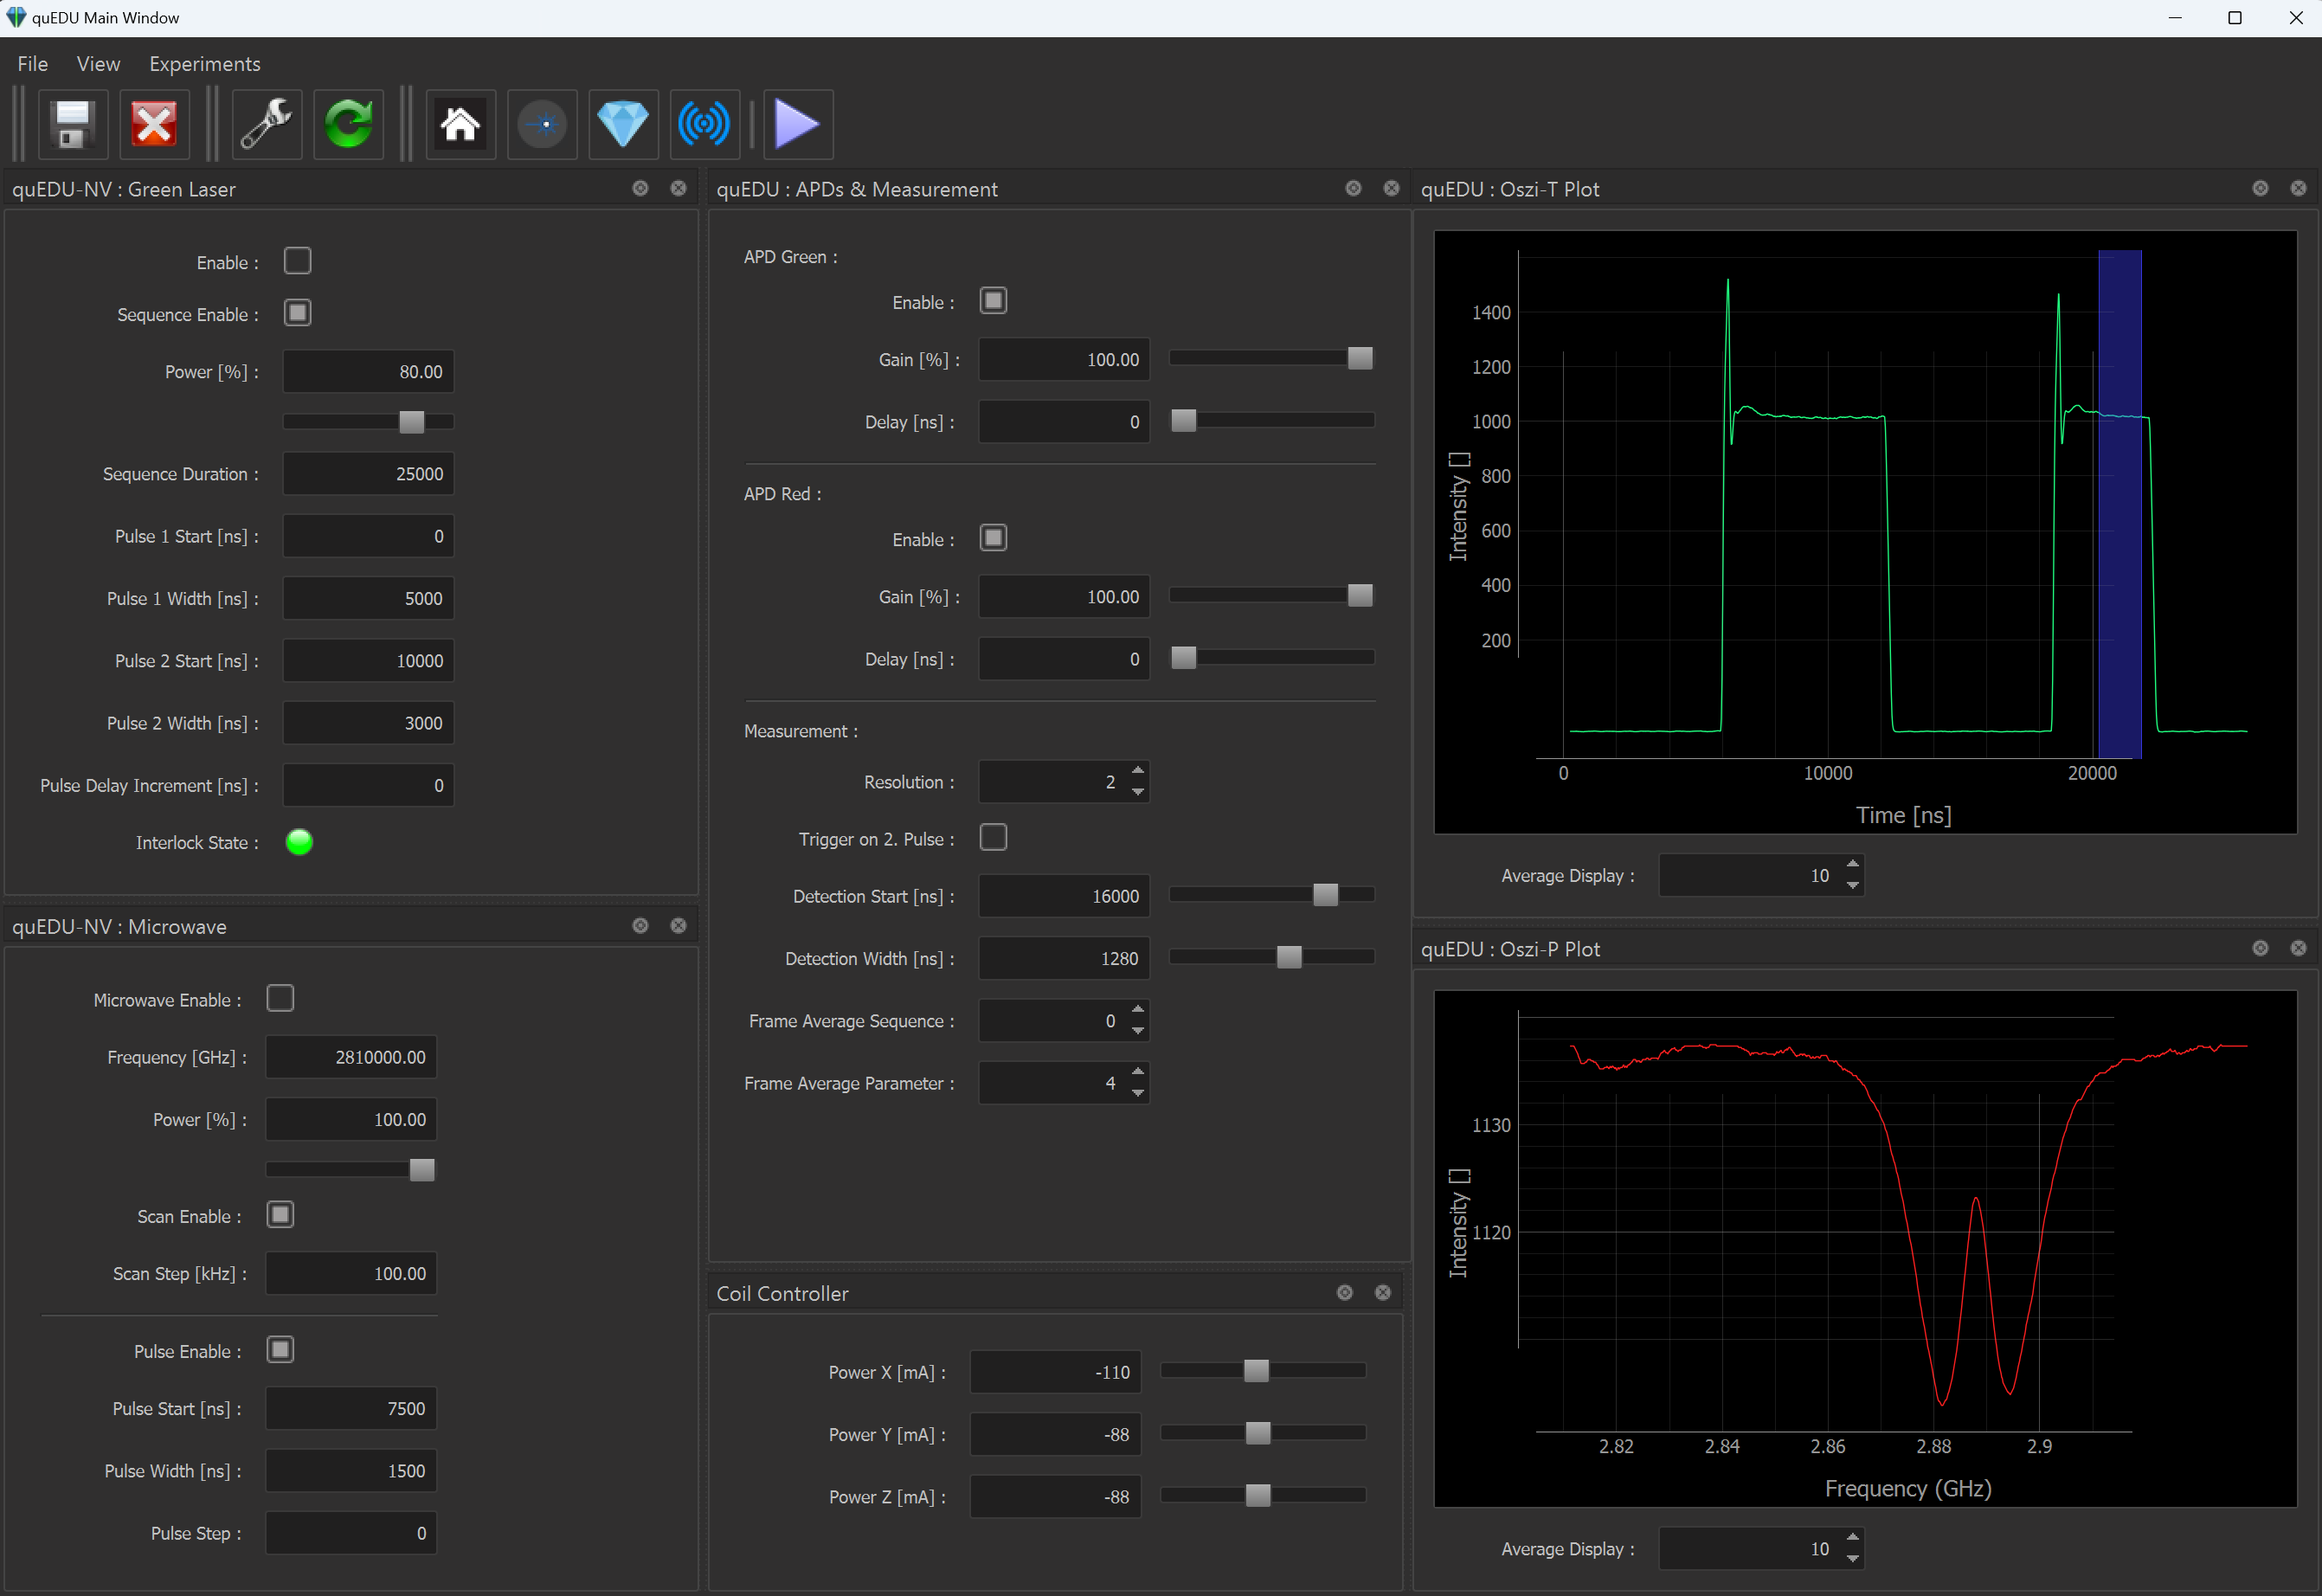
\includegraphics[width=1.0\textwidth]{gfx/diagrams/ODMR_pythonGUI.png}
	\caption{\acs{ODMR} visualization} 
	\label{fig:4.12}
\end{figure}

The blue rectangle on the Oszi-T plot delineates the detection window within which an \acs{ODMR} dip is observed in the Oszi-P plot. Users have the option to increase the detection width and adjust its position through the \acs{APD}s and Measurement dock widget. The parameters for average display and resolution can be utilized to reduce noise within the spectrum, thereby yielding a smoother representation of the plot. Furthermore, by varying the microwave power—accomplished through adjustments in the current of the coils via the coil controller dock widget—one may observe multiple dips within the Oszi-P plot. This is illustrated in Fig \ref{fig:4.6}